\section{Project description}
\label{chapter1}

The Project description section provides a brief overview of the project, covering the basic idea with simple sketches for visualization.

\subsection{Problem desription}

%FIXME: De-uglify diagram (Lorenzo)

The aim of the project is to develop a simplified adaptive cruise control (ACC) system based on two Raspberry Pi 4 devices communicating with each other via Bluetooth. Node 1 is responsible for collecting environmental data using ultrasonic sensors, while Node 2 controls the vehicle speed and interacts with the user via a touch display.

\begin{figure}[h]
	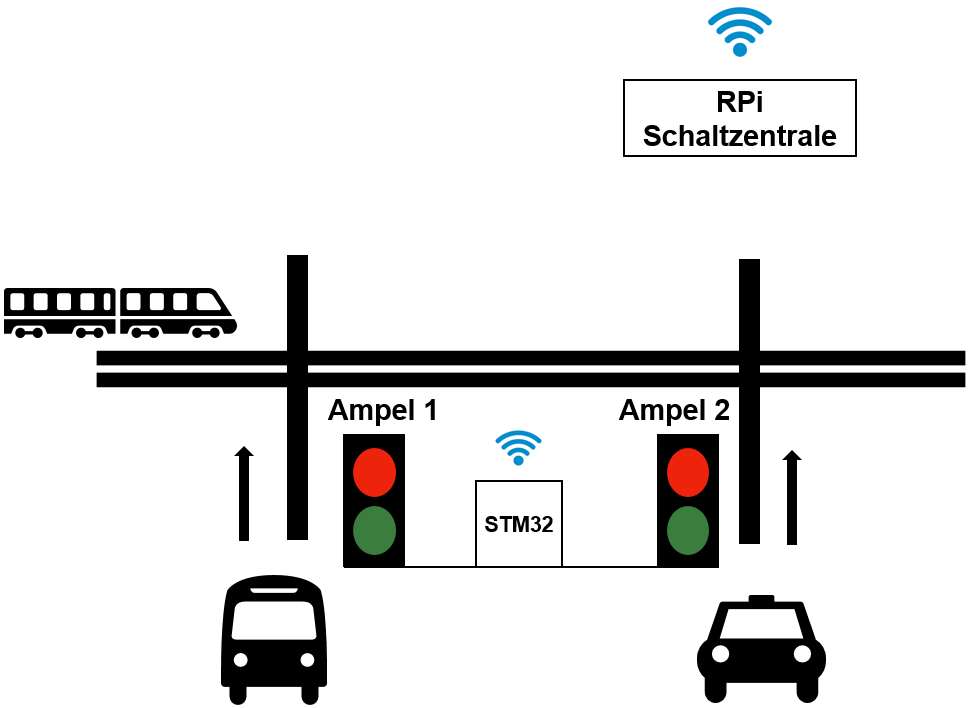
\includegraphics[height=100mm]{images/system}
	\centering
	\caption{system description}
	\label{fig:system}
\end{figure}

\paragraph{}
%The adaptive cruise control (acc) system consists of two nodes, node1, and node2. The nodes are connected by a (FIXME: encrypted/authenticated/both) bluetooth link.

\paragraph{}
Node 1 is equipped with two HC-SR04 ultrasonic sensors that detect obstacles in front of a virtual vehicle. At the request of Node 2, Node 1 performs measurements with both sensors, checks their results for consistency and plausibility, and then transmits the validated values to Node 2. In addition to the distance data, the response message also contains information about the status of the consistency and plausibility check. The error assumption is that at most one of the two sensors can fail within a defined period of time. Node 1 is designed to act fail-silent in the event of a fault: it does not deliver faulty measured values to Node 2, but suppresses the output in case of doubt and does not transmit any data at all if both sensors are faulty.
%FIXME: The fault hypothesis is that one of these sensors can fail, but not both of them within a defined time span. We design node1 in such a way that it is fail-silent: It does not convey incrrect readings to node2, but it may convey no readings at all if the sensors are failing.

\paragraph{}
Node 2 takes over the function of the steering control unit (ECU) of the virtual vehicle. A control panel on the display can be used to increase or decrease the speed of the vehicle, while an additional switch turns the adaptive cruise control (ACC) system on or off. The display shows the current speed and the operating status of the ACC (active/inactive) and emits an alarm message in the event of a fault. The requirements for status display, speed display, alarm messages, and user input can be conveniently implemented using a touchscreen display, for example, with a corresponding \href{https://www.berrybase.at/raspberry-pi-touch-display-2-7-portrait} {Raspberry Pi-compatible device}. 

%node2 represents the steering wheel ECU of the virtual car. It is connected to a control panel by which the virtual vehicle can be accelerated/decelerated. Another switch turns the adaptive cruise control on or off. A display shows the current speed of the car and gives status information on whether acc is on or off. Moreover it shows an alarm if the acc detects an error. FIXME: We can solve the status/speed/alarm/input requirements with a touch screen, e.g. \href{https://www.berrybase.de/3-5-ips-display-fuer-raspberry-pi-mit-resistivem-touchscreen} {such a device}.

\paragraph{}
\textbf{Hardware used:}
\begin{itemize}
    \item 2 × Raspberry Pi 4B
    \item 2 × HC-SR04 Ultraschallsensor
    \item 1 × Raspberry Pi Touch Display 2, 7" Portrait
\end{itemize}
